\documentclass[12pt,a4paper]{report}
\usepackage[utf8]{inputenc}
\usepackage[inner=3.5cm,outer=2.5cm,bottom=3cm,top=2.5cm,pdftex]{geometry}
\usepackage{setspace}
\usepackage{graphicx}
\usepackage{rotating}
\usepackage[page]{appendix}
\usepackage{float}
\usepackage[font=small,labelfont=bf]{caption}
\usepackage{subfigure}
\usepackage{titlesec}
\usepackage[hidelinks]{hyperref}
\usepackage{listings}
\usepackage{textcomp}
\usepackage{fancyhdr}
\usepackage{multirow}
\usepackage{verbatim}	%makes it possible to comment out a section of text by using \begin{comment}...\end{comment}
\usepackage[table,xcdraw]{xcolor}
\usepackage{pifont}
\usepackage{mathptmx}
\usepackage{wrapfig}
\usepackage{ragged2e}
\usepackage[nottoc,notlot,notlof]{tocbibind}
\usepackage[norsk]{babel}

\definecolor{involvecolor}{RGB}{0,206,209}

% Style chapter headings for preface and toc.
\setlength{\headheight}{15pt}
\titlespacing*{\chapter}{0pt}{0pt}{4ex}
\titleformat{\chapter}[display]
 {\bfseries\Large}
 {}
 {0pt}
 {\color{involvecolor}\titlerule[2.0pt]\vspace{2ex}\filright\color{black}}
 [\color{involvecolor}\vspace{2ex}{\titlerule[2.0pt]}]


\setstretch{1.25}
\begin{document}
{\RaggedRight
\pagestyle{fancy}

% empty default settings for fancy layout
\fancyhf{}

% table mark commands
\newcommand{\cmark}{\textcolor{green!80!black}{\ding{51}}}
\newcommand{\xmark}{\textcolor{red}{\ding{55}}}
\newcommand{\plusmark}{\textcolor{green!80!black}{\textbf{+}}}
\newcommand{\minusmark}{\textcolor{red}{\textbf{-}}}

% chapter, section, header and footer layout
\renewcommand{\sectionmark}[1]{\markright{\thesection ~ \ #1}}
\renewcommand{\chaptermark}[1]{\markboth{ #1}{}}
\renewcommand{\headrulewidth}{0.5pt}
\renewcommand{\footrulewidth}{0.5pt}

%head setting
%\fancyhead[L]{\textcolor{black} {\rightmark}}
\fancyfoot[C]{\textcolor{black} {\thepage}}

% Redefine the plain page style - used when the page is a chapter
\fancypagestyle{plain}{%
  \fancyhf{}%
  \renewcommand{\headrulewidth}{0pt}% Line at the header invisible
  \renewcommand{\footrulewidth}{0.5pt}% Line at the footer visible
  \fancyfoot[C]{\textcolor{black} {\thepage}}
}

% Avoid hyphenating
\tolerance=10
\emergencystretch=\maxdimen
\hyphenpenalty=10000
\hbadness=10000

\pagenumbering{roman}
\chapter*{Sammendrag}
\textit{ Hvordan kan Involve ved hjelp av kommunikasjon og effektiv ledelse forbedre muligheten for å nå virksomhetens mål?} 


\setcounter{tocdepth}{2}
\tableofcontents
\addtocontents{toc}{~\hfill\textbf{Side}\par}

% ----------- CHAPTERS ----------------

% Parts
\cleardoublepage
% Style chapter one with involve image.
\titleformat{\chapter}[display]
 {\bfseries\Large}
 {}
 {0pt}
 {\color{involvecolor}\titlerule[2.0pt]\vspace{2ex}\filright\color{black}}
 [\color{involvecolor}\vspace{0ex}{\titlerule[2.0pt]}]
\pagenumbering{arabic}
\setcounter{page}{1}
\chapter[Innledning]{
\includegraphics[scale=0.5]{bilder/logo.png}}
\section{Motivasjon for oppgaven}
Da vi startet studien ønsket vi å undersøke betydningen av effektiv ledelse, og hvordan ledelse kan påvirke de ansattes evne? til å jobbet mot en felles visjon og målsetting. Ledere har et overordnet ansvar med tanke på å sørge for motiverte medarbeidere som jobber sammen mot et felles mål. Karismatiske ledere inspirerer medarbeiderne til å overta lederens tenkning, væremåte og  ånd når denne ikke er tilstede, og jobber kontinuerlig med effektiv internkommunikasjon.(Brønn og Arnulf s137). Internkommunikasjon handler om hvordan ulike grupper og avdelinger i organisasjonen knyttes sammen gjennom kommunikasjon. I et strategisk perspektiv påvirker internkommunikasjon virksomhetens evne til å skape samhandling, utvikling, motivasjon og trivsel - faktorer som er viktige for en vellykket drift (estudie).

\section{Problemstilling}
Problemstillingen ble utarbeidet gjennom innledende samtaler med kommunikasjonsrådgiver Kjetil væhle (tidligere daglig leder) og tilgang til en tidligere medarbeiderundersøkelse som ble gjennomført i januar 2019. De viktigste funnene fra undersøkelsen var en manglende tillit til ledelsens måte å drive virksomheten på og ledelsens evne til å skape motivasjon. Undersøkelsen ga også inntrykk av utfordringer knyttet til samarbeid og kommunikasjon på tvers av avdelinger. (informasjon om samarbeid kom fra samtaler, ikke undersøkelse) 

\indent \newline
De innledende samtalene med Kjetil Væhle ga oss i tillegg informasjon om at virksomheten ikke har klart å nå de finansielle målsettingene de siste årene. På bakgrunn av denne informasjonen kom vi frem til følgende problemstilling:
\textit{Hvordan kan Involve ved hjelp av kommunikasjon og effektiv ledelse forbedre muligheten for å nå virksomhetens mål?} 

\section{Om bedriften}
Involve er et relativt nytt kommunikasjonshus med bred kompetanse innenfor reklame og PR. Selskapet vokste frem som et resultat av flere fusjoner i 2011, og er en del av Havas, et internasjonalt reklame- og kommunikasjonsnettverk. De drives som et selvstendig norskeid byrå, hvor arbeidsoppgavene retter seg mot PR, design, reklame, markedsføring m.m. Filosofien baserer seg på navnet til virksomheten og handler om å skape produkter og tjenester som engasjerer og involverer målgruppen. Virksomheten består av fire avdelinger; Pro-X, Advertising, PR og Xpress.

\indent \newline
Kommunikasjonsbransjen er inne i en utvikling som kjennetegnes av økt digitalisering og en økning i tempo. Konkurransen blant aktørene anses som svært tøff, hvor oppdragene ofte blir lagt ut som åpne anbud. Prosjekter for kundene krever tverrfaglig kompetanse, og flere fagdisipliner må dermed samarbeide for å kunne levere et konkurransedyktig produkt. Dette fører til at det stilles sterkere krav til internkommunikasjonen enn tidligere. 


% Style chapter headings.
\titleformat{\chapter}[display]
 {\bfseries\Large}
 {}
 {0pt}
 {\color{involvecolor}\titlerule[2.0pt]\vspace{2ex}\filright\color{black} \thechapter . }
 [\color{involvecolor}\vspace{2ex}{\titlerule[2.0pt]}]
\chapter{Teoretisk forankring}
I dette kapittelet vil vi kort redegjøre for teoretiske modeller og rammeverk som vil bli benyttet i oppgaven. Med utgangspunkt i disse teoriene vil vi analysere ledelsen til Involve, og se hva ledelsen kan gjøre annerledes for å skape bedre forutsetninger for å nå virksomhetens mål.

\section{Koorienteringsmodellen}
Modellen til Mcleod og Chaffee (1973) har til hensikt å forklare hvordan kommunikasjonsproblemer kan oppstå som følge av ulik tolkning og oppfatning blant en leder og interessenter. Modellen bruker fire assosiasjonstyper som definerer og påvirker interaksjonen mellom partene; forståelse, enighet, samsvar og nøyaktighet \cite[s.~157]{KommunikasjonForLedere}. I følge Dozier og Ehling (1992) er det fire koorienteringstilstander partene kan befinne seg i, hvor de to sistnevnte skaper konflikter;

\begin{itemize}
\item\textit{Sann konsensus} - Partene er enige om å være enige
\item\textit{Dissens} - Partene er enige om å være uenige
\item\textit{Falsk konsensus} - Partene er uenige, men tror de er enige
\item\textit{Falsk konflikt} - Partene er enige, men tror de er uenige
\end{itemize}

Modellen illustrerer hvor lett misforståelser kan føre til konflikter i situasjoner hvor lederen ikke er oppmerksom på om deres oppfatning av de ansattes synspunkter er nøyaktig \cite[s.~158]{KommunikasjonForLedere}. I oppgaven har vi benyttet modellen med et formål om å analysere situasjoner i virksomheten som hindrer effektiv ledelse og kommunikasjon.

\section{Makt, styring og ledelse}
Ledelse blir ofte blandet sammen med begreper som makt, styring og autoritet. For å kunne gjennomføre nøyaktige analyser angående Involve sin ledelse, finner vi det hensiktsmessig å definere begrepene, og hvordan ledelse skiller seg fra tradisjonell styring og makt. Makt handler om å påtvinge andre sin egen vilje, og tvinge folk til en bestemt livsførsel. Styring tar for seg selve kjernen i organisering, det vil si regler, prosedyrer, rutiner og systemer. Autoritet er knyttet til personer og betegner enkeltpersoners rett til å utøve styring. I motsetning til disse begrepene, dreier ledelse seg om å skape oppslutning fra folk som prinsipielt kunne villet noe annet, og å mobilisere innsatsvilje og samarbeid mot et felles mål \cite[s.~130]{KommunikasjonForLedere}.

\indent \newline
Med utgangspunkt i ovennevnte definisjon av ledelse, vil neste avsnitt presentere ledelsesteorier som legges til grunn for å besvare problemstillingen. 

\section{Transformasjonsledelse og transaksjonsledelse}
Transformasjonsledelse er moderne ledelsesteorier som har vokst frem i løpet av de siste 40 årene, og bygger på Max Webers gamle begrep karisma \cite[s.~137]{KommunikasjonForLedere}. Karisma handler om lederens evne til å inspirere, motivere og appellere til hvert enkelt individs følelsesmessige behov. Det er ansett som en viktig attributt for å lykkes med transformasjonsledelse. Ledere som oppfattes som karismatiske, vil bygge tillit hos de ansatte og et ønske om å ville identifisere seg med lederen \cite[s.~75]{PerspektiverLedelse}.

\indent \newline
Transformasjonsledere evner å utvide og stimulere ansattes interesser gjennom å skape tilhørighet til virksomhetens konkrete og overordnede mål. Samtidig påvirkes ansatte til å se utover sine egne interesser \cite[s.~75]{PerspektiverLedelse}. Det finnes flere ulike teorier om transformasjonsledelse, men vi har valgt å fokusere på Bernard Bass sin tolkning av teorien. Bass forklarer teorien gjennom fire dimensjoner som omhandler transformasjonslederens karisma. Disse er;

\begin{itemize}
\item\textit{Idealisert innflytelse} - Omhandler lederens evne til å kommunisere verdier og visjoner ved å opptre som en inspirerende rollemodell. Lederen evner å skape innflytelse hos de ansatte gjennom sine handlinger.
\item\textit{Inspirerende motivasjon} - Lederen inspirerer og motiverer medarbeiderne gjennom å skape tilhørighet til felles mål og delte visjoner. Lederen snakker om fremtiden med tiltro til mestring.
\item\textit{Intellektuell stimulering} - Lederen fremmer kreativitet og innovativ atferd blant medarbeiderne. De ansatte føler seg oppmuntret til å arbeide selvstendig med oppgavene og finne nye kreative løsninger på problemer.
\item\textit{Individuelle hensyn} - Medarbeidernes behov for måloppnåelse og vekst blir hensyntatt, og lederen bidrar med støttende, læringsorientert og personlig samhandling.
\end{itemize}
\cite{inspirerendeLeder}

\indent \newline
Til sammenligning med transformasjonsledelse, der ansattes inspirasjon og motivasjon skal komme innenfra, handler transaksjonsledelse om inspirasjon fra ytre faktorer. For arbeidstakeren oppfattes arbeidsforholdet som en transaksjon der man tilbyr arbeidskraft i bytte mot lønn. Arbeidsforholdet kjennetegnes også av mindre personlige relasjoner mellom leder og medarbeiderne.

\indent \newline
To fremtredende kjennetegn ved transaksjonsledelse er \textit{betinget belønning} og \textit{ledelse ved unntak} \cite[s.~76]{PerspektiverLedelse}. Betinget belønning går ut på at arbeidstaker blir lovet belønning for de resultatene de oppnår. Ledelse ved unntak skiller mellom \textit{aktiv} og \textit{passiv} ledelsesstil. Lederen kan gå aktivt inn og lete etter avvik på rutiner og prosedyrer og gripe inn, eller han/hun kan velge å passivt følge med og kun si fra dersom regler ikke blir fulgt. 

\indent \newline
Begge ledelsesteoriene kan danne grunnlag for suksess, men det er transformasjonsledelse som vil kunne danne grunnlag for motiverte medarbeidere som jobber mot et felles overordnet mål. Teoriene er ikke gjensidig utelukkende, og lederen kan kjennetegnes med egenskaper fra begge ledelsesstilene. 



\chapter{Metode}
Metode handler om hvordan man innhenter informasjon, og hvordan data skal analyseres og tolkes. Videre er det vanlig å dele metodelære inn i to hovedmetoder;
\begin{itemize}
\item\textit{Kvantitativ metode} - Befatter seg med tall og det som er målbart (kvantifiserbart). (wiki - kvant. metode). Metoden gir en høy grad av generaliserbarhet basert på tallfestet data. En rask og oversiktlig metode for å innhente kvantitativ data på er gjennom spørreundersøkelser. En svakhet ved spørreundersøkelser er imidlertid faren ved å overse informasjon som ikke kan tallfestes. Dette kan føre til at informasjonen gir et overfladisk og forenklet bilde av virkeligheten.
\item\textit{Kvalitativ metode} - Generering av kunnskap basert på menneskelig erfaring og fortolkning, og brukes ofte til å undersøke sosiale prosesser og sosialt samspill (ref blanding av wiki - Kval. met og Etikkom). En av de vanligste teknikkene for innhenting av kvalitative data er ved intervjuer. Teknikken benyttes for å sikre en dypere forståelse for emnet man ønsker å undersøke.
\end{itemize}

I oppgaven har vi benyttet begge metodene for å generalisere funnene og samtidig få en dypere forståelse av årsakene som ligger bak. 

\section{Datainnsamling}
Prosessen i datainnsamlingen startet med uformelle samtaler med tidligere daglig leder, nå kommunikasjonsrådgiver, Kjetil Væhle. Ett av gruppemedlemmene kjente Væhle fra før, og det var derfor naturlig å benytte denne relasjonen til å få grunnleggende informasjon om virksomheten og markedet den opererer i. Videre fikk vi tidlig i prosessen tilgang til sekundærdata i form av en medarbeiderundersøkelse som hadde blitt gjennomført i januar 2019 (se vedlegg?). Undersøkelsen ga inntrykk av utfordringer knyttet til ledelsen. På bakgrunn av undersøkelsen og de innledende samtalene fikk vi utarbeidet den aktuelle problemstillingen, og innhentet videre primærdata gjennom en spørreundersøkelse og to dybdeintervjuer. I tillegg har vi gjennom hele arbeidsprosessen hatt mulighet til å kontakte Væhle ved behov.

\section{Spørreundersøkelse}
Spørreundersøkelsen ble gjennomført av 15 ansatte via web (Qualtrics). Spørreskjemaet bestod av 8 spørsmål med 5 tilhørende svaralternativer, hvor spørsmålene var formulert som påstander. Respondentene kunne velge en score fra 1 (svært uenig) til 5 (svært enig), basert på deres oppfatning om den aktuelle påstanden. 

\section{Dybdeintervjuer}
Dybdeintervjuene ble gjennomført på bakgrunn av spørreundersøkelsen, for å få en dypere innsikt og forståelse for resultatene. Vi benyttet en semistrukturert intervjuform hvor samtalen mellom forskeren og intervjuobjektet blir styrt av forskeren. Intervjuobjektene bestod av en medarbeider som jobber i Advertising (ønsket å være anonym) og tidligere daglig leder Kjetil Væhle. I begge tilfeller åpnet vi intervjuene med å be objektene fortelle og dele generelle tanker og oppfatninger av dagens ledelse. Tanken bak dette var å skape en åpen samtale og anledning for deltakerne til å snakke fritt om emnet, uten påvirkning fra spørsmålsstillerne. Utover i intervjuene stilte vi spørsmål knyttet til resultatene fra spørreundersøkelsen og emnene vi ønsket å få en dypere innsikt i. Begge intervjuene ble foretatt separat i Involve sine lokaler.

\section{Refleksjoner rundt validitet, pålitelighet og generaliserbarhet}
Validitet handler om gyldighet, og om man på bakgrunn av resultatene av en studie kan trekke gyldige slutninger om det man ønsker å undersøke (validitet SNL). For å sikre en høy grad av validitet har vi innhentet data gjennom kvantitative - og kvalitative undersøkelser. Det kan imidlertid stilles spørsmålstegn ved generaliserbarheten, da kun 15 av 32 mulige respondenter besvarte den kvantitative spørreundersøkelsen. I forhold til pålitelighet har vi bevisst valgt å innhente primærdata fra begge parter. I tillegg har kontaktpersonen vår i Involve vært en god kilde til datainnsamling i forhold til å se problemstillingen fra både ledernes- og medarbeidernes perspektiv. 

\chapter{Resultater og funn}
Under vil vi presentere relevante funn og resultater relatert til problemstillingen. Data er hentet gjennom spørreundersøkelsen og dybdeintervjuene.

\indent \newline
Undersøkelsen er utarbeidet gjennom ledelsesteori presentert tidligere i oppgaven. Formålet er å vurdere dagens ledelse ved Involve. Resultatene er som følger:

\begin{figure}[H]
\centering
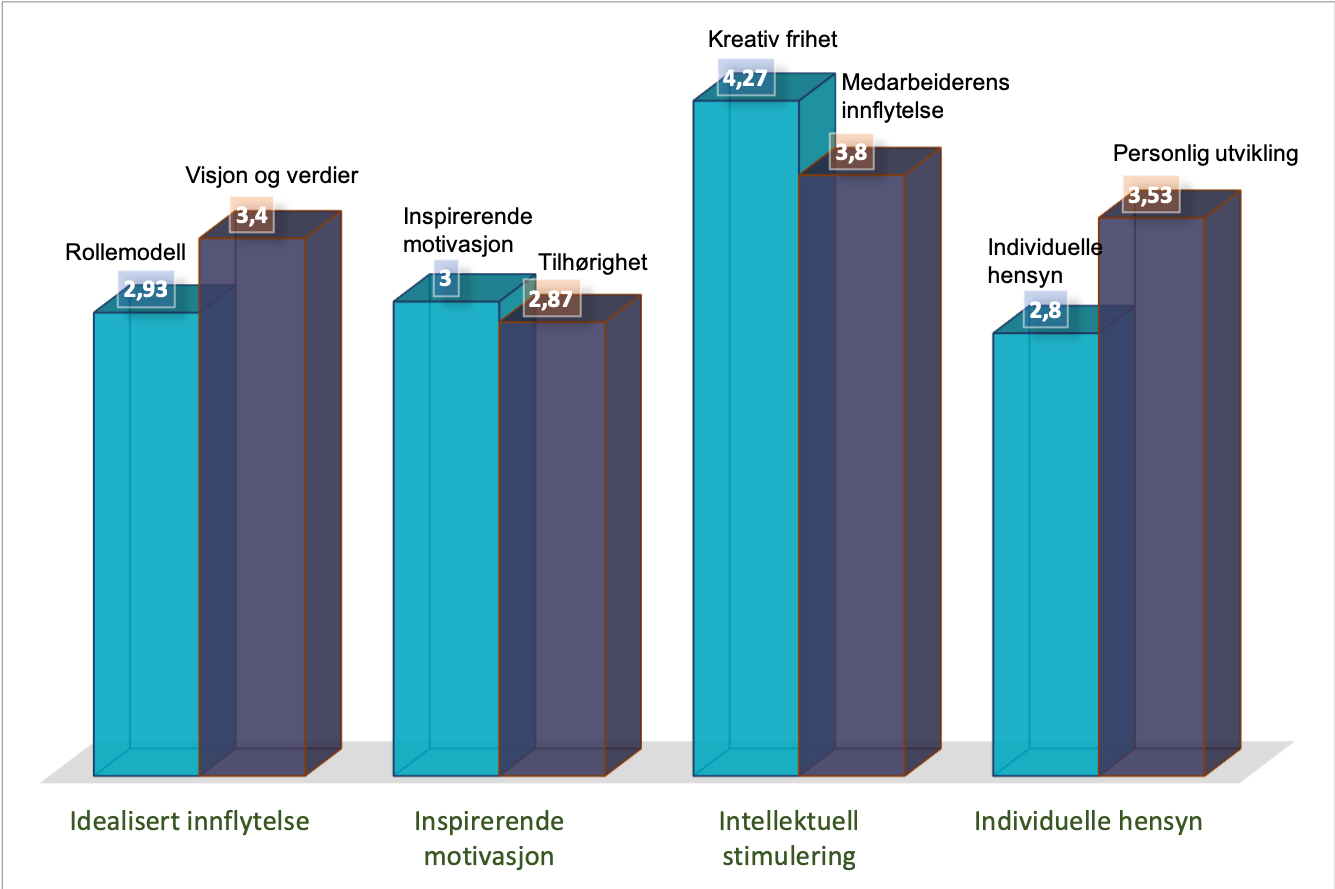
\includegraphics [scale=0.6]{bilder/resultat.png}
\caption{Spørreundersøkelse - resultat}
\label{fig:resultat}
\end{figure}

\begin{itemize}
\item\textit{Idealisert innflytelse} -  Lederens evne til å opptre som rollemodell og formidle visjoner og verdier gjennom egne handlinger.
\begin{itemize}
\item\textit{Rollemodell} - 2,93 av 5,00 hvorav 80\% enten var nøytrale (3), uenig (2) eller svært uenig (1).
\item\textit{Visjon og verdier} -  3,4 av 5,00 hvorav 53\% enten var nøytrale (3), uenig (2) eller svært uenig (1).
\end{itemize}
Dybdeintervjuet viste til at medarbeiderne oppfatter lederne som hardtarbeidende, men retter for lite oppmerksomhet mot medarbeiderne.

\item\textit{Inspirerende motivasjon} - Lederens evne til å inspirere og motivere ved å skape tilhørighet til felles mål og ambisjoner.
\begin{itemize}
\item\textit{Motivasjon} - 3,00 av 5,00 hvorav 73\% enten var nøytale (3), uenig (2) eller svært uenig (1).
\item\textit{Tilhørighet} - 2,87 av 5,00 hvorav 73\% enten var nøytale (3), uenig (2) eller svært uenig (1). 
\end{itemize}

\item\textit{Intellektuell stimulering} - Lederens evne til å fremme kreativitet og innovativ atferd.
\begin{itemize}
\item\textit{Individuelle hensyn} - 2,80 av 5,00 hvorav 87\% enten var nøytrale (3), uenig (2) eller svært uenig (1).
\item\textit{Personlig utvikling} - 3,53 av 5,00 hvorav 47\% enten var nøytrale (3), uenig (2) eller svært uenig (1). 
Årsaken til dette ble forklart av medarbeideren som en konsekvens av lite tilstedeværelse blant de ansatte, grunnet stress og fokus på kunder.
\end{itemize}

\item\textit{Individuelle hensyn} - Lederens evne til å samhandle og ta hensyn til individuelle behov for måloppnåelse og vekst.
\begin{itemize}
\item\textit{Kreativ frihet} - 4,27 av 5,00 hvorav 13\% enten var nøytrale (3), uenig (2) eller svært uenig (1). 
\item\textit{Inkludering ved viktige avgjørelser} - 3,80 av 5,00 hvorav 33\% var nøytale (3), uenig (2) eller svært uenig (1).
Intervjuobjektet (medarbeideren) beskrev de ansatte som tilfredse med ledernes evne til å oppfordre til kreativitet. I en del tilfeller blir imidlertid kreativitet begrenset grunnet budsjettrammer.
\end{itemize}
\end{itemize}

\indent \newline
På spørsmål knyttet til transaksjonsledelse fortalte Væhle at Involve ikke opererer med noe bonussystem i dag, og at dette heller ikke er vanlig for lignende bedrifter. 

\indent \newline
Avslutningsvis i begge intervjuene stilte vi spørsmål om det er andre utfordringer virksomheten burde ta tak i. Medarbeideren forklarte at de ansatte i perioder føler arbeidsmengden er for stor. Dette medfører at de blir tildelt prosjekter og arbeidsoppgaver som de ikke føler de behersker godt nok. Vi kontaktet Væhle ved en senere anledning for å forhøre oss om ledelsen er oppmerksomme på dette problemet. I følge hans oppfatning har ledelsen ikke blitt informert om dette, og er dermed ikke klar over medarbeidernes oppfatning angående arbeidsmengden. 

\indent \newline
Væhle fortalte i sitt intervju om utfordringer knyttet til samarbeid mellom avdelingene. Avdelingene blir holdt adskilt, i den forstand at hver enkelt avdeling har egne målsettinger og budsjetter å etterfølge. 


\chapter{Analyse}
Under vil vi diskutere funnene fra spørreundersøkelsen og dybdeintervjuene, og gjennom teori analysere resultatene opp mot problemstillingen. Til slutt vil vi gi anbefalinger relatert til hva virksomheten kan gjøre annerledes og områder ledelsen bør forbedre for å øke sannsynligheten for å nå virksomhetens mål.

\section{Konflikt mellom ledelsen og de ansatte}
Basert på intervjuene har vi identifisert uenighet mellom ledelsen og medarbeiderne med tanke på arbeidsmengden. Ledelsen mener at arbeidsmengden ikke oppleves som unormalt høy og at den er nødvendig for å levere resultatene de ønsker. De begrunner dette med et tøft marked hvor de må gripe prosjektmulighetene de får. I motsetning til ledelsen mener medarbeiderne at arbeidsmengden er for stor, og fører enkelte ganger til at de må utføre arbeidsoppgaver de ikke behersker godt nok. Ledelsen er ikke klar over at de ansatte mener arbeidsmengden er for stor, samtidig som at medarbeiderne tror ledelsen deler samme oppfatning som dem.

\begin{figure}[H]
\centering
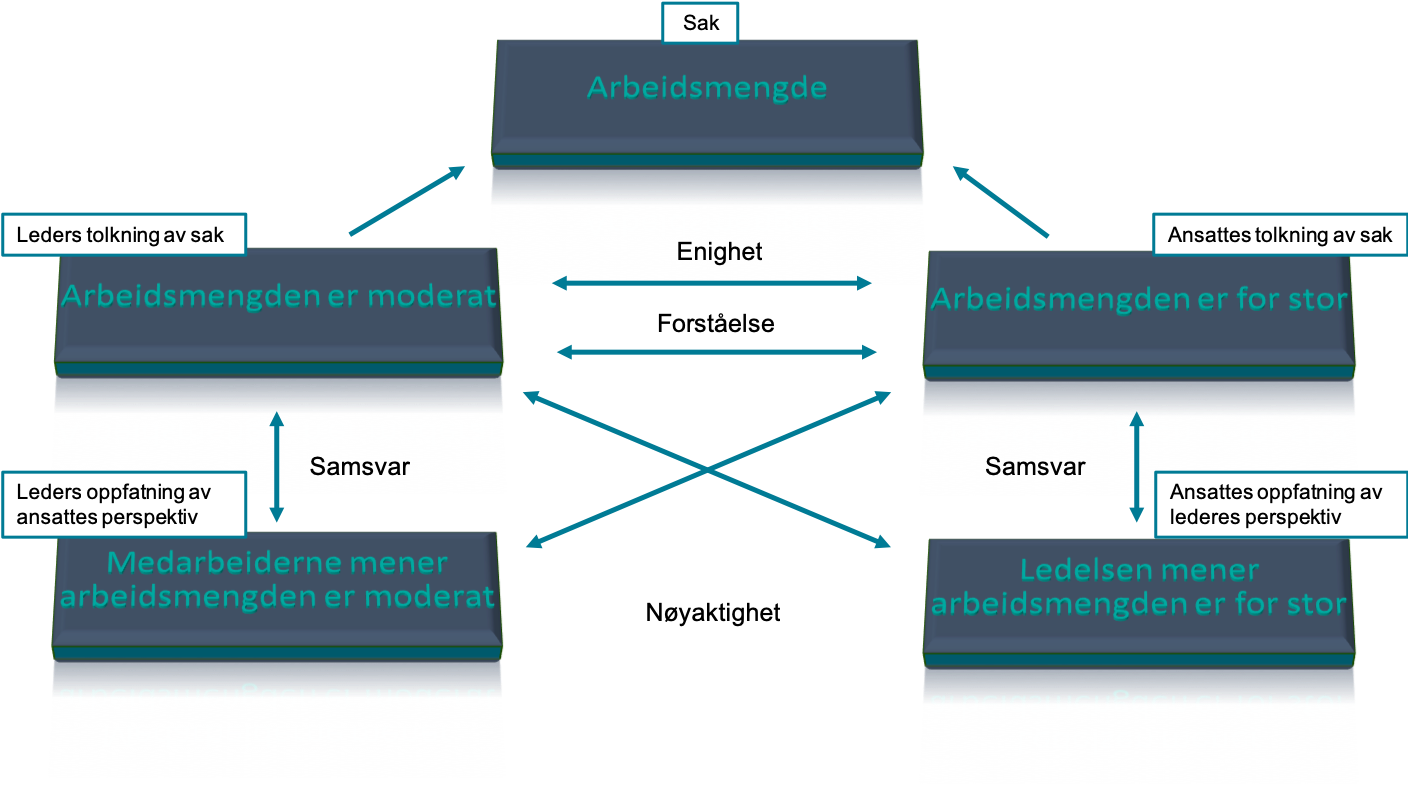
\includegraphics [scale=0.6]{bilder/koo.png}
\caption{Koorienteringsmodellen - arbeidsmengde}
\label{fig:koo}
\end{figure}

Koorienteringsmodellen viser at partene befinner seg i tilstanden som omtales som falsk konsensus. Den reflekterer én av to tilstander som tilsier at partene er i konflikt. Partene tror de er enige, men i virkeligheten er de uenige. I utgangspunktet er det positivt med utfordrende oppgaver, hvor lederen oppmuntrer de ansatte til kreativ problemløsning, og til å finne løsninger på problemer selv. Men i dette tilfellet føler medarbeiderne behov for hjelp og veiledning.

\indent \newline
Konflikten påvirker mestringsfølelsen hos de ansatte, og virker negativt inn på motivasjonen. En annen konsekvens er at det kan føre til at Involve leverer et svakere sluttprodukt til kundene. Dette kan påvirke lønnsomheten på sikt. På bakgrunn av analysen vil vi derfor oppfordre ledelsen til å tilbringe mer tid sammen med de ansatte, og veilede ved behov. 

\section{Effektiv ledelse}
I oppgaven har vi definert ledelse som evnen til å skape oppslutning fra folk som prinsipielt kunne villet noe annet, og å mobilisere innsatsvilje og samarbeid mot et felles mål. I tillegg fant vi det hensiktsmessig å skille ledelse fra makt, styring og autoritet. For å avgjøre om Involve praktiserer effektiv ledelse i dag, har vi basert analysen vår på teori om transformasjonsledelse og transaksjonsledelse.

\subsection{Transformasjonsledelse}
En av de viktigste oppgavene til en leder er å formidle felles mål og visjoner som sørger for at alle interessentene i virksomheten jobber mot det samme overordnede målet. Basert på vår analyse har ikke ledelsen klart å henge med i utviklingen innenfor kommunikasjonsbransjen, hvor mange av prosjektene krever samarbeid mellom avdelingene. Med for mye fokus på målsettinger innenfor hver enkelt avdeling, skapes det dårlige rammevilkår for et godt samarbeid mellom de ulike grupperingene i virksomheten. En slik suboptimalisering vil kunne føre til at de ansatte jobber mot resultater som vil gagne deres avdeling, men som ikke nødvendigvis er optimalt for virksomheten totalt sett. Ledelsen bør derfor definere en tydeligere visjon og felles målsetting, samtidig som hver enkelt avdelingsleder jobber med å kommunisere disse. Fokus på dette området vil kunne skape bedre forutsetninger for effektivt samarbeid og ansatte som jobber mot en felles retning og visjon.

\indent \newline
Dimensjonen som omhandler lederens evne til å fremme kreativitet og innovativ adferd var den dimensjonen med høyest score i spørreundersøkelsen. Gjennom analysene våre kommer det frem at ledelsen er flinke til å gi de ansatte kreativt spillerom, uten å blande seg inn i utførelsen av prosjektene. Dette er en viktig faktor for å skape selvstendighet og personlig utvikling. 

\indent \newline
Gode personlige relasjoner er med på å skape samhold og bidrar til å gjøre medarbeiderne mer stolte og forpliktet til arbeidsplassen sin. Selv om ledernes evne til å fremme kreativitet og innovativ adferd oppleves som god, viser funnene knyttet til samhandling, måloppnåelse og ansattes vekst, en ledelse som benytter for mye tid på eksterne interessenter. Ledelsen evner ikke å etablere personlige forhold til sine ansatte. Dette kan ses i sammenheng med mangel på veiledning. Ved å være mer direkte involvert i arbeidsoppgavene vil lederne knytte personlige bånd, samtidig som de får innsikt i personlige mål og ambisjoner hos de ansatte. Det vil være viktig at de finner en god balanse, slik at dette ikke går på bekostning av kreativ - og innovativ frihet.

\subsection{Transaksjonsledelse}
Fra resultatene relatert til transformasjonsledelse fremgår det at lederne tenderer mot å benytte en passiv ledelsesstil. Istedenfor å skape personlige relasjoner med de ansatte, velger ledelsen i for stor grad å passivt følge med og kun si ifra dersom regler og prosedyrer ikke blir fulgt. I følge Bernard Bass er dette en oppskrift på middelmådighet  \cite[s.~74]{PerspektiverLedelse}.

\indent \newline
Funnene viser videre at ledelsen ikke har for vane å motivere de ansatte ved bruk av bonuser. I følge medarbeideren har ledelsen tidligere iverksatt individuelle bonusordninger, men det ble ikke tatt godt imot blant de ansatte. Årsaken til dette er at det skapte konkurranse internt i virksomheten, i tillegg til at målene føltes uoppnåelige. Motivasjonen ble påvirket negativt og bonussystemet virket derfor mot sin hensikt. Bonussystemer kan i utgangspunktet fungere som et motivasjonsinsentiv. For Involve kan en mulighet være å benytte seg av bonusordninger på tvers av avdelinger, som har fokus på å belønne team-baserte prestasjoner. 

\section{Anbefalinger}
Analysene viser at dagens utøvelse av ledelse er en mellomting av transformasjonsledelse, transaksjonsledelse og styring, med hovedvekt på de to sistnevnte ledelsesstilene. Lederne har for lite fokus på å skape personlige relasjoner med de ansatte, samt skape motivasjon og inspirasjon til å jobbe mot felles mål. For at Involve skal effektivisere ledelsen, og dermed potensielt forbedre mulighetene for å nå målsettingene, anbefaler vi følgende:

\begin{itemize}
\item Utarbeide et tydelig overordnet mål på tvers av avdelingene som avdelingslederne sørger for å kommunisere jevnlig til medarbeiderne.
\item Avsette mer tid sammen med de ansatte for å skape personlige relasjoner og lære om enkeltindividers personlige mål og behov for vekst.
\item Tilby hjelp og veiledning når medarbeiderne jobber med utfordrende oppgaver som tærer på motivasjon og mestringsfølelsen.
\item Eventuelle bonusordninger bør innføres på bakgrunn av team-baserte prestasjoner.
\end{itemize}



\chapter{Konklusjon}
Oppgaven har hatt som formål å undersøke hvordan ledelsen ved Involve fungerer, og besvare problemstillingen \textit{Hvordan kan Involve ved hjelp av kommunikasjon og effektiv ledelse forbedre muligheten for å nå virksomhetens mål?} 

\indent \newline
Vurdering av effektiv ledelse er blitt gjennomført ved å definere begrepet ledelse, og gjennom teori relatert til transaksjonsledelse og transformasjonsledelse, med spesielt fokus på Bernard Bass sine fire dimensjoner. 

\indent \newline
På bakgrunn av analysen kan vi konkludere med at virksomheten ikke praktiserer effektiv ledelse i stor nok grad. Vi oppfordrer ledelsen til å fokusere på ovennevnte anbefalinger for å utvikle seg innenfor dimensjonene; idealisert innflytelse, inspirerende motivasjon, intellektuell stimulering og individuelle hensyn. Forbedringer på disse områdene vil kunne resultere i inspirerte og motiverte ansatte, som jobber mot en felles visjon og større muligheter for at Involve når fremtidige målsettinger.
 
% chapter heading as preface and toc
\titleformat{\chapter}[display]
 {\bfseries\Large}
 {}
 {0pt}
 {\color{involvecolor}\titlerule[2.0pt]\vspace{2ex}\filright\color{black}}
 [\color{involvecolor}\vspace{2ex}{\titlerule[2.0pt]}]
 
\renewcommand\bibname{Referanseliste}
\bibliographystyle{apalike}	% (uses file "plain.bst")
\bibliography{mineReferanser}		% expects file "mineReferanser.bib"
}

\end{document}
